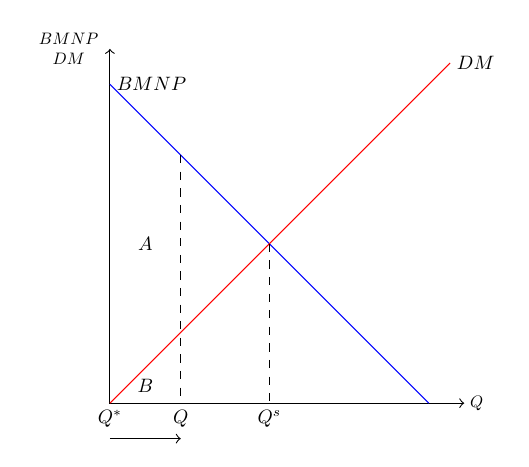
\begin{tikzpicture}[scale=0.9]
% Ejes
\draw[<->] (0,5)  node [text width=15mm,text centered, scale=0.6, left] {$BMNP$ $DM$}-- (0,0) -- (5,0) node [scale=0.6, right] {$Q$};

% Rectas
\draw[blue] (0,4.5) node [right, scale=0.7, black] {$BMNP$} -- (4.5,0);
\draw[red] (0,0)  node [below, scale=0.7, black] {$Q^\ast$} -- (4.8,4.8) node [right, scale=0.7, black] {$DM$};

% Rectas sombreadas
\draw[dashed] (1,3.5) -- (1,0)  node [below, scale=0.7, black] {$Q$};
\draw[dashed] (2.25, 2.25) -- (2.25,0) node [below, scale=0.7, black] {$Q^s$};

% A y B
\draw (0.5,2.25) node [scale=0.7, black] {$A$};
\draw (0.5,0.25) node [scale=0.7, black] {$B$};

% Flechas
\draw[->] (0,-0.5) -- (1,-0.5);
\end{tikzpicture}